
\section{RepairingStrategy : Taint Analysis}
\label{sec:taintAnalysis}

We have used taint analysis to detect program paths between source-sink pair in
the program to determine which variables and objects go to tainted sink like
database, print stream, network stream etc. We have used InfoFlow framework and
modify it for our usage. The detaild design of the taint analysis module is
given in Chapter~\ref{chapter:SystemDesign}
Section~\ref{subsubsec:TaintingRule}. 

\subsection{Taint analysis : Definition}
\label{subsec:TaintAnalysisDef}

The term \textbf{taint} in the aspect of programming language is defined as
below:
\begin{definition}
Set of variables which are associated with program input is the set of tainted
variables.
\end{definition}
\begin{definition}
Variables which are associated or referenced from tainted variables are also
tainted.
\end{definition}
So, the set of variables are called as \textbf{tainted variable set} which may
trigger some undesirable events in the application.

\subsection{Taint analysis : Taint Propagation}
\label{subsec:TaintPropagation}

All tainted variables do not possess security threat. The tainted problem is
defined at three points. They are:

\begin{enumerate}
	\item Source descriptor $<m,n_s,p_s>$
	\item Derivation descriptor $<m,n_d,p_d>$
	\item Sink descriptor $<m,n_s,n_d,p_s,p_d>$
\end{enumerate}
Where $m$ is the method, $n$ is the number of parameter(s), $p$ is the access
path.$s$ and $d$ denotes to source and sink(destination) respectively.
\begin{figure}[ht!]
\centering
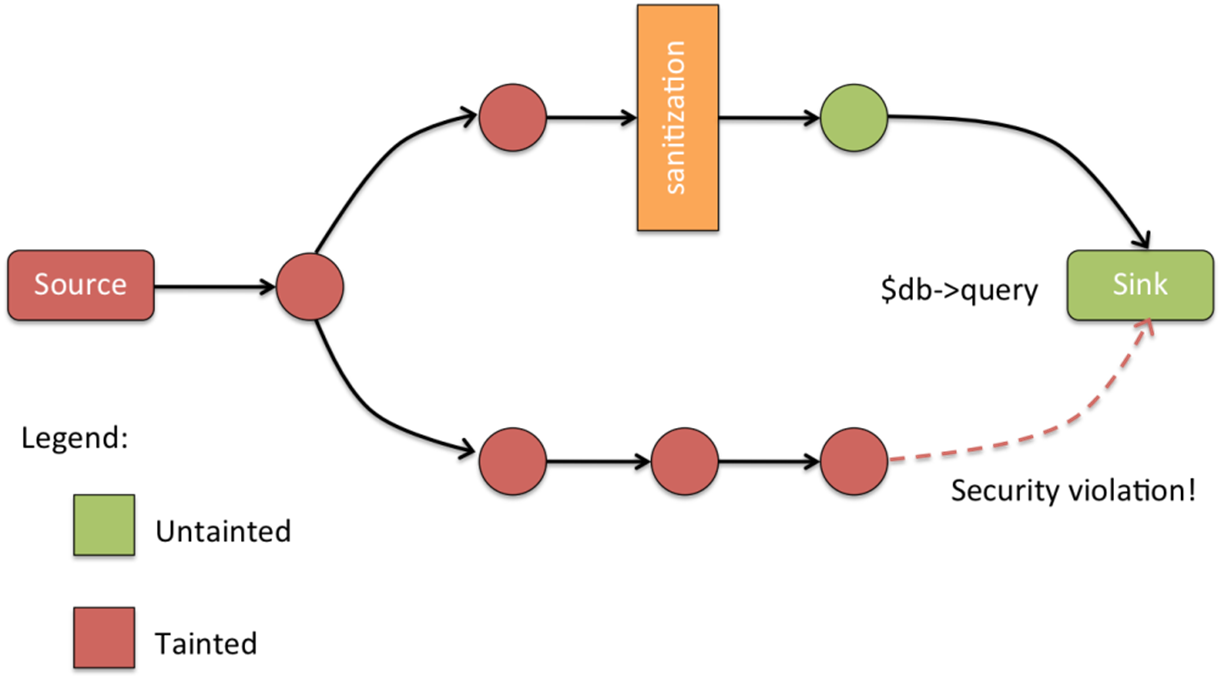
\includegraphics[width=5.5in]{images/Taint.png}
\caption{A simplified diagram indicating taint problem}
\label{fig:taint}
\end{figure}

\subsection{Taint Analysis : Relevance with Repairing Effort}
\label{subsec:TaintRepairing}

We have considered static taint analysis of the program (here we are analyzing
only java byte code) to eliminate any possibility of patching on the statements
which may go to some tainted sink like database, print stream or network stream.
Doing such we can ensure that the variables and objects we are patching will be
contained inside the system thus will not be leaked to outside. On such example
can be a client application on which we have done patching. Assume that we
patched a string object which was given as a input to the program. Due to some
formatting problem, the program throws a runtime exception. Ins uch scenario we
will regenerate the string object according to the constraint in the program to
make sure it stays very close to a clean input string. in any case the generated
string goes out from the system and used as a input to any external module it
may causes problem as the patched sting was solely designed for that particular
program. 

To avoid such cases we analyze the statement which in in the path of potential
tainted source and sink. In such cases we would not patch such statements.
